\documentclass[sigconf]{acmart}
\settopmatter{printacmref=false} % Removes citation information below abstract
\renewcommand\footnotetextcopyrightpermission[1]{} % removes footnote with conference information in first column
\pagestyle{plain} % removes running headers

\usepackage{booktabs}
\usepackage{setspace}
\usepackage{listings}
\usepackage{courier}
\usepackage{enumitem}
\usepackage{multirow}
\usepackage{color}
\usepackage{xcolor}
\usepackage{totpages}

\let\oldthebibliography=\thebibliography
\let\endoldthebibliography=\endthebibliography
\renewenvironment{thebibliography}[1]{
  \begin{oldthebibliography}{#1}
    \setlength{\parskip}{0ex}
    \setlength{\itemsep}{0ex}
}
{
  \end{oldthebibliography}
}

\sloppy

\newcommand{\mm}{mm$^2$}
\newcommand{\figtitle}[1]{\textbf{#1}}
\newcommand{\us}{$\mu$s}
\newcommand{\fixme}[1]{{\color{red}\textbf{#1}}}

\definecolor{pink}{rgb}{1.0,0.47,0.6}
\newcommand{\adrian}[1]{{\color{green}\textbf{#1}}}
\newcommand{\laura}[1]{{\color{pink}\textbf{#1}}}
\newcommand{\joel}[1]{{\color{red}\textbf{#1}}}
\newcommand{\ameen}[1]{{\color{blue}\textbf{#1}}}
\newcommand{\arup}[1]{{\color{yellow}\textbf{#1}}}
\newcommand{\hungwei}[1]{{\color{purple}\textbf{#1}}}


\newcommand{\note}[2]{\fixme{$\ll$ #1 $\gg$ #2}}

\newcommand{\myitem}[1]{\item \textbf{#1}}

\newcommand{\horizbar}{\rule{\linewidth}{.5mm}}
\newcommand{\app}[1]{{\sc #1}}
 
\renewcommand{\em}{\it}

  
\newcommand{\BigO}[1]{${\cal O}(#1)$}
\newcommand{\BigOmega}[1]{$\Omega(#1)$}
\newcommand{\BigTheta}[1]{$\Theta(#1)$}
 
\newcommand{\ceiling}[1]{\left\lceil #1 \right\rceil}
\newcommand{\faM}{\lfloor \alpha M \rfloor}
%\newcommand{\C}[2]{{#1 \choose #2}}

\newcommand{\x}{$\times$}
 
%\newcommand{\comment}[1]{}
\newcommand{\ignore}[1]{}


%\newcommand{\boldparagraph}[1]{\vspace*{-0ex}\paragraph{#1}}
\newcommand{\boldparagraph}[1]{\vspace*{1ex}\noindent\textit{#1}\hspace{1em}}

%%%%% SINGLE FIGURE
\def\cfigure[#1,#2,#3]{
\begin{figure}
\vspace*{0mm}
\begin{center}

\includegraphics[width=3in]{#1} 
 
\vspace*{-3mm}\caption[]{#2
} \label{#3}
 
\vspace*{-5mm}
\end{center}
%\horizbar
%\vspace*{-2mm}
\end{figure}}

%%%%% SINGLE FIGURE 4in wide
\def\cfigurefour[#1,#2,#3]{
\begin{figure}
\vspace*{0mm}
\begin{center}

\includegraphics[width=4in]{#1} 
 
\vspace*{-3mm}\caption[]{#2
} \label{#3}
 
\vspace*{-5mm}
\end{center}
%\horizbar
%\vspace*{-2mm}
\end{figure}}

%%%%% SINGLE FIGURE
\def\cfiguretemp[#1,#2,#3]{
\begin{figure}
\vspace*{0mm}
\begin{center}

\includegraphics[width=3.5in]{#1} 
 
\vspace*{-3mm}\caption[]{#2
} \label{#3}
 
\vspace*{-5mm}
\end{center}
%\horizbar
\vspace*{-2mm}
\end{figure}}

%%%%% SINGLE WIDE FIGURE
\def\wfigure[#1,#2,#3]{
\begin{figure*}
\vspace*{0mm}
\begin{center}
 \includegraphics[width=\textwidth]{#1} 
 \vspace*{-3mm}\caption[]{#2
} \label{#3}
 
\end{center}
%\horizbar
\end{figure*}}

%%%%% 3 FIGURES IN A ROW
\def\threefigure[#1,#2,#3,#4,#5]{
\begin{figure*}
\vspace*{0mm}
\begin{center}

\begin{tabular}{ccc}
\includegraphics[width=2in]{#1} & \includegraphics[width=2in]{#2} &  \includegraphics[width=2in]{#3} \\
(a) & (b) & (c) \\
\end{tabular}

\vspace*{-3mm}\caption[]{#4
} \label{#5}

\vspace*{-5mm}
\end{center}
%\horizbar
\vspace*{-2mm}
\end{figure*}}

%%%%%% DOUBLE FIGURE
\def\dcfigure[#1,#2,#3,#4,#5,#6]{
{
\begin{figure*}
\begin{center}
\begin{minipage}[c]{\columnwidth}{
\includegraphics[width=\columnwidth]{#1} 
\vspace*{0mm}\caption[]{#2} \label{#3} \
}\end{minipage}\hspace*{\columnsep}\
\begin{minipage}[c]{\columnwidth}{
\includegraphics[width=\columnwidth]{#4} 
\vspace*{0mm}\caption[]{#5}\label{#6} \
}\end{minipage}
\end{center}
\end{figure*}
}
}


\def\tableByTable[#1,#2,#3,#4,#5,#6]{
{
\begin{table*}
\begin{center}
\begin{minipage}[c]{3in}{
\centering
{#1}
\vspace*{0mm}\tabcaption[]{#2}\label{#3} \
}\end{minipage}\hspace*{\columnsep}\
\begin{minipage}[c]{3in}{
\centering
{#4}
\vspace*{0mm}\tabcaption[]{#5}\label{#6} \
}\end{minipage}
\end{center}
\end{table*}
}
}


\def\figureByTable[#1,#2,#3,#4,#5,#6]{
{
\begin{figure*}
\begin{center}
\begin{minipage}[c]{3in}{
\centering
\includegraphics[width=\textwidth]{#1}
\vspace*{0mm}\figcaption[]{#2} \label{#3} \
}\end{minipage}\hspace*{\columnsep}\
\begin{minipage}[c]{3.3in}{
\centering
{#4}
\vspace*{0mm}\tabcaption[]{#5}\label{#6} \
}\end{minipage}
\end{center}
\end{figure*}
}
}

\def\tableByFigure[#1,#2,#3,#4,#5,#6]{
{
\begin{figure*}
\begin{center}
\begin{minipage}[c]{4.3in}{
\centering
{#1}
\vspace*{0mm}\tabcaption[]{#2} \label{#3} \
}\end{minipage}\hspace*{\columnsep}\
\begin{minipage}[c]{2.2in}{
\centering
\includegraphics[width=\textwidth]{#4}
\vspace*{-0.35in}\caption[]{#5}\label{#6} \
}\end{minipage}
\end{center}
\end{figure*}
}
}

% two figs pdfs in one column fig
\def\doublecfigure[#1,#2,#3,#4]{
{
\begin{figure}
\begin{center}
\begin{minipage}[c]{1.5in}{
\begin{center}
\includegraphics[width=1.5in]{#1}%\\(a)
\end{center}
}\end{minipage}\hspace*{1em}\
\begin{minipage}[c]{1.5in}{
\begin{center}
\includegraphics[width=1.5in]{#2}%\\(b)
\end{center}
}\end{minipage}
\vspace*{0mm}\caption[]{#3} \label{#4} \
\end{center}
\end{figure}
}
}

\def\qcfigure[#1,#2,#3,#4,#5,#6]{
{
\begin{figure*}
\vspace*{0.2in}\
\begin{center}
\begin{minipage}[c]{3in}{
\includegraphics[width=3in]{#1} 
\vspace*{-3mm}
}
\end{minipage}\hspace*{0.5in}\
\begin{minipage}[c]{3in}{
\includegraphics[width=3in]{#2} 
\vspace*{-3mm}
}\end{minipage}

\begin{minipage}[c]{3in}{
\includegraphics[width=3in]{#3} 
\vspace*{-3mm}
}
\end{minipage}\hspace*{0.5in}\
\begin{minipage}[c]{3in}{
\includegraphics[width=3in]{#4} 
\vspace*{-3mm}
}\end{minipage}
\end{center}
\caption[]{#5}\label{#6}
\end{figure*}
}
}

\def\twfigure[#1,#2,#3,#4,#5]{
{
\begin{figure*}
\vspace*{0.2in}\
\begin{center}
\begin{minipage}[c]{6.5in}{
\includegraphics[width=6.5in]{#1} 
\vspace*{-3mm}
}
\end{minipage}

\begin{minipage}[c]{6.5in}{
\includegraphics[width=6.5in]{#2} 
\vspace*{-3mm}
}\end{minipage}

\begin{minipage}[c]{6.5in}{
\includegraphics[width=6.5in]{#3} 
\vspace*{-3mm}
}
\end{minipage}
\end{center}
\caption[]{#4}\label{#5}
\end{figure*}
}
}

\def\dwfigure[#1,#2,#3,#4]{
{
\begin{figure*}
\vspace*{0.2in}\
\begin{center}
\begin{minipage}[c]{6.5in}{
\includegraphics[width=6.5in]{#1} 
\vspace*{-3mm}
}
\end{minipage}

\begin{minipage}[c]{6.5in}{
\includegraphics[width=6.5in]{#2} 
\vspace*{-3mm}
}\end{minipage}

\end{center}
\caption[]{#3}\label{#4}
\end{figure*}
}
}



\def\dssfigure[#1,#2,#3,#4,#5,#6]{
{
\begin{figure*}
\vspace*{0.2in}\
\begin{center}
\begin{minipage}[c]{4in}{
\includegraphics[width=4in]{#1}
\vspace*{-3mm}\caption[]{#2} \label{#3} \
}\end{minipage}\hspace*{0.5in}\
\begin{minipage}[c]{2in}{
\includegraphics[width=2in]{#4}
\vspace*{-3mm}\caption[]{#5}\label{#6} \
}\end{minipage}
\end{center}
\vspace*{-0.4in}\
\end{figure*}
}
}




\def\dsfigure[#1,#2,#3,#4,#5,#6]{
{
\begin{figure*}
\vspace*{0.2in}\
\begin{center}
\begin{minipage}[c]{3in}{
\includegraphics[width=3in]{#1}
\vspace*{-3mm}\caption[]{#2} \label{#3} \
}\end{minipage}\hspace*{0.5in}\
\begin{minipage}[c]{3in}{
\hspace*{0.5in}\
\includegraphics[height=3in]{#4}
\vspace*{-3mm}\caption[]{#5}\label{#6} \
}\end{minipage}
\end{center}
\vspace*{-0.4in}\
\end{figure*}
}
}


\def\dsyfigure[#1,#2,#3,#4,#5,#6]{
{
\begin{figure*}
\vspace*{0.2in}\
\begin{center}
\begin{minipage}[c]{2.5in}{
\includegraphics[height=2.5in]{#1}
\vspace*{-3mm}\caption[]{#2} \label{#3} \
}\end{minipage}\hspace*{0.5in}\
\begin{minipage}[c]{2.5in}{
\includegraphics[height=2.5in]{#4}
\vspace*{-3mm}\caption[]{#5}\label{#6} \
}\end{minipage}
\end{center}
\vspace*{-0.4in}\
\end{figure*}
}
}

\def\dyfigure[#1,#2,#3,#4,#5,#6]{
{
\begin{figure*}
\vspace*{0.2in}\
\begin{center}
\begin{minipage}[c]{3in}{
\includegraphics[height=3in]{#1} 
\vspace*{-3mm}\caption[]{#2} \label{#3} \
}\end{minipage}\hspace*{0.5in}\
\begin{minipage}[c]{3in}{
\includegraphics[height=3in]{#4} 
\vspace*{-3mm}\caption[]{#5}\label{#6} \
}\end{minipage}
\end{center}
\vspace*{-0.4in}\
\end{figure*}
}
}

%%%%%% DOUBLE FIGURE Y
\def\dyoldfigure[#1,#2,#3,#4,#5,#6]{
{
\begin{figure*}
\vspace*{0.2in}\
\begin{center}
\begin{minipage}[c]{3in}{
\epsfysize=2.0in\
\hspace{0.5in}\
\epsfbox{#1}
\vspace*{-3mm}\caption[]{#2} \label{#3} \
}\end{minipage}\hspace*{0.25in}\
\begin{minipage}[c]{3in}{
\epsfysize=2.0in\
\hspace{0.5in}\
\epsfbox{#4}
\vspace*{-3mm}\caption[]{#5}\label{#6} \
}\end{minipage}
\end{center}
\vspace*{-0.4in}\
\end{figure*}
}
}

%%%%%% DOUBLE FIGURE Y IN A COLUMN!!
\def\cfiguredouble[#1,#2,#3,#4]{
\begin{figure}
\vspace*{0.2in}\
\begin{center}
\begin{minipage}[c]{1.5in}{
\epsfxsize=1.5in\
\epsfbox{#1}
}\end{minipage}\hspace*{0.1in}\
\begin{minipage}[c]{1.5in}{
\epsfxsize=1.5in\
\vspace{0.1in}\epsfbox{#2}
}\end{minipage}\vspace*{-0.10in} \caption[]{#3}\label{#4}
\end{center}
\vspace*{-0.4in}\
\end{figure}
}


%%%%% Single programmable size figure
\def\wpfigure[#1,#2,#3,#4]{
\begin{figure*}
\vspace*{4mm}
\begin{center}

\includegraphics[width=#4]{#1} 

\vspace*{-3mm}\caption[]{#2
} \label{#3}

\vspace*{-5mm}
\end{center}
%\horizbar
\end{figure*}}

%%%%% Single programmable size figure, rotated
\def\wprfigure[#1,#2,#3,#4,#5]{
\begin{figure*}
\vspace*{4mm}
\begin{center}

\includegraphics[width=#4, angle=#5]{#1} 

\vspace*{-3mm}\caption[]{#2
} \label{#3}

\vspace*{-5mm}
\end{center}
%\horizbar
\end{figure*}}




%%%%% Adjacent, programmable-width figures, slid vertically by 9th
%%%%% parameter
\def\DoubleFigureWSlide[#1,#2,#3,#4,#5,#6,#7,#8,#9]{
\begin{figure*}
\vspace*{#9}
\begin{center}
\begin{minipage}{#4}
\includegraphics[width=#4]{#1}
\vspace*{-3mm}\caption{#2
}\label{#3}
\end{minipage}
\hspace{2em}
\begin{minipage}{#8}
\includegraphics[width=#8]{#5}
\vspace*{-3mm}\caption{#6
}\label{#7}
\end{minipage}
\vspace*{-5mm}
\end{center}
\end{figure*}
}


%%%%% Adjacent, programmable-width figures
\def\DoubleFigureW[#1,#2,#3,#4,#5,#6,#7,#8]{
\begin{figure*}
\vspace*{0in}
\begin{center}
\begin{minipage}{#4}
\includegraphics[width=#4]{#1}
\vspace*{-3mm}\caption{#2
}\label{#3}
\end{minipage}
\hspace{2em}
\begin{minipage}{#8}
\includegraphics[width=#8]{#5}
\vspace*{-3mm}\caption{#6
}\label{#7}
\end{minipage}
\vspace*{-5mm}
\end{center}
\end{figure*}
}



\def\DoubleFigureWHack[#1,#2,#3,#4,#5,#6,#7,#8]{
\begin{figure*}
\vspace*{0in}
\begin{center}
\begin{minipage}{3in}
\includegraphics[width=#4]{#1}
\vspace*{-3mm}\caption{#2
}\label{#3}
\end{minipage}
\hspace{2em}
\begin{minipage}{3in}
\includegraphics[width=#8]{#5}
\vspace*{-3mm}\caption{#6
}\label{#7}
\end{minipage}
\vspace*{-5mm}
\end{center}
\end{figure*}
}






%%%%%% DOUBLE FIGURE
\def\ddcfigure[#1,#2,#3,#4]{
\begin{figure*}
\vspace*{0.2in}\
\begin{center}
\begin{minipage}[c]{\columnwidth}{
\includegraphics[width=\columnwidth]{#1} 
}\end{minipage}\hspace{0.5in}\
\begin{minipage}[c]{\columnwidth}{
\includegraphics[width=\columnwidth]{#2} 
}\end{minipage} \caption[]{#3}\label{#4}
\end{center}
\end{figure*}
}

\def\ddcfigureSlide[#1,#2,#3,#4,#5]{
\begin{figure*}
\vspace*{#5}\
\begin{center}
\begin{minipage}[c]{3in}{
\includegraphics[height=3in]{#1} 
}\end{minipage}\hspace{0.5in}\
\begin{minipage}[c]{3in}{
\includegraphics[height=3in]{#2} 
}\end{minipage}\vspace*{-0.10in} \caption[]{#3}\label{#4}
\end{center}
\vspace*{-0.4in}\
\end{figure*}
}

\def\cxfigure[#1,#2,#3]{
\begin{figure}
\vspace*{4mm}
\begin{center}
 
\epsfxsize=2.5in\
\epsfbox{#1}\
 
\vspace*{-0.10in}\caption[]{#2
} \label{#3}
 
\vspace*{-5mm}
\end{center}
%\horizbar
\vspace*{-2mm}
\end{figure}}

\newenvironment{panefigure}{\begin{figure}\begin{center}}{\end{center}\end{figure}}

\newcommand{\pdfpane}[3]{
\begin{minipage}{#1}
\begin{center}
\includegraphics[width=#1]{#2}\\(#3)
\end{center}
\end{minipage}
}

\newcommand{\figWidth}{\columnwidth}
\newcommand{\figSep}{0.05in} 
%\newcommand{\figSep}{\columnsep} 
\newcommand{\figWidthOne}{3.05in} 
\newcommand{\figWidthHalf}{5.85in} 
\newcommand{\figWidthTwo}{3.7in} 
\newcommand{\figWidthThree}{2in} 
\newcommand{\figWidthFour}{1.3in} 
\newcommand{\figWidthFive}{2.3in} 
\newcommand{\figWidthSix}{2.3in} 
\newcommand{\figHeight}{2.0in}
\newcommand{\figHeightOne}{2.6in}
\newcommand{\captionText}[2]{\textbf{#1} \textit{\small{#2}}}

\newcommand{\beforecaption}{\vspace{-.15cm}\begin{spacing}{0.85}}
\newcommand{\aftercaption}{\vspace{-.45cm}\end{spacing}}
% \newcommand{\mycaption}[3]{{\beforecaption\caption{\label{#1}\footnotesize{\textbf{#2}} {\em #3}}\aftercaption}}
% haryadi, change mycaption three to mycaptionthree
%\newcommand{\mycaption}[3]{{\caption[#2]{{\bf #2.} {\em #3}}\label{#1}}}
%\newcommand{\mycaption}[3]{\beforecaption\caption{\label{#1}{\small \bf #2} \em\scriptsize #3}\aftercaption}
%\newcommand{\mycaption}[3]{\beforecaption\caption{\label{#1}{\bf #2} \em\footnotesize #3}\aftercaption}
\newcommand{\mycaption}[3]{\caption{\label{#1}{\bf #2} \em\small #3}}


%%%%% general

% only foreign words should be italicized... (example given should not)
\newcommand{\eg}{\textit{e.g.}}
\newcommand{\ie}{\textit{i.e.}}
\newcommand{\etal}{\textit{et al.}}
\newcommand{\etc}{\textit{etc.}}
\newcommand{\adhoc}{\textit{ad hoc}}

% units
\newcommand{\KB}{\,KB}
\newcommand{\MB}{\,MB}
\newcommand{\GB}{\,GB}
\newcommand{\TB}{\,TB}
\newcommand{\GBs}{\,GB/s}
\newcommand{\MBs}{\,MB/s}
\newcommand{\KBs}{\,KB/s}
\newcommand{\Kbs}{~Kbit/s}
\newcommand{\gbps}{\,Gbps}
\newcommand{\mbs}{~Mbit/s}
\newcommand{\mus}{\mbox{$\mu s$}}
\newcommand{\ms}{\mbox{$ms$}}

%\newcommand{\fsync}{\texttt{fsync}}

% axes
\newcommand{\xaxis}{x-axis}
\newcommand{\yaxis}{y-axis}


\newcommand{\unix}{{\sc Unix}}
\newcommand{\NULL}{{\sc NULL}}
\newcommand{\sysread}{\texttt{read}}
\newcommand{\syssync}{\texttt{sync}}
\newcommand{\fsync}{\texttt{fsync}}
\newcommand{\syswrite}{\texttt{write}}
\newcommand{\sysseek}{\texttt{lseek}}
\newcommand{\sysstat}{\texttt{stat}}
\newcommand{\make}{\texttt{make}}
\newcommand{\ioctl}{\texttt{ioctl}}
\newcommand{\panic}{\texttt{panic}}
\newcommand{\truncate}{\texttt{truncate}}
\newcommand{\rmdir}{\texttt{rmdir}}
\newcommand{\unlink}{\texttt{unlink}}
\newcommand{\open}{\textit{open}}
\newcommand{\close}{\textit{close}}
\newcommand{\linkscount}{\texttt{linkscount}}
\newcommand{\msync}{\textit{msync}}
\newcommand{\mmap}{\textit{mmap}}
\newcommand{\unmap}{\textit{munmap}}
\newcommand{\map}{\textit{map}}
\newcommand{\fetch}{\textit{gfetch}}
\newcommand{\acquire}{\textit{acquire}}
\newcommand{\commitxact}{\textit{commit}}
\newcommand{\commit}{\textit{commit}}
\newcommand{\barrier}{\textit{thread-barrier}}


% dsnvm
\newcommand{\dsnvm}{DSPM}
\newcommand{\dsm}{DSM}
\newcommand{\nvm}{PM}
\newcommand{\hotpot}{Hotpot}
\newcommand{\mrmw}{MRMW}
\newcommand{\mrsw}{MRSW}
\newcommand{\wfetch}{FETCH}
\newcommand{\cd}{CD}
\newcommand{\dr}{DR}
\newcommand{\on}{ON}
\newcommand{\dn}{DN}
\newcommand{\xn}{CN}
\newcommand{\master}{MN}
\newcommand{\xactid}{CID}
\newcommand{\dirty}{dirty}
\newcommand{\committed}{committed}
\newcommand{\redundant}{redundant}
\newcommand{\ib}{IB}
\newcommand{\sendreply}{\texttt{send-reply}}
\newcommand{\atomicsendreply}{\texttt{atomic-send-reply}}
\newcommand{\multisendreply}{\texttt{multicast-send-reply}}
\newcommand{\journaled}{JOURNALED}
\newcommand{\fsyncsafe}{FSYNC\_SAFE}
\newcommand{\X}{{$\times$}}
\newcommand{\pmfs}{PMFS}
\newcommand{\tmpfs}{tmpfs}
\newcommand{\Octopus}{Octopus}
\newcommand{\Mojim}{Mojim}
\newcommand{\dsmnoxact}{DSM-NoXact}
\newcommand{\dsmxact}{DSM-Xact}
\newcommand{\clflush}{\texttt{clflush}}
\newcommand{\pcommit}{\texttt{pcommit}}
\newcommand{\mfence}{\texttt{mfence}}
\newcommand{\sfence}{\texttt{sfence}}
\newcommand{\ra}{\textbf{R1.a}}
\newcommand{\rb}{\textbf{R1.b}}
\newcommand{\rcs}{\textbf{R2.a}}
\newcommand{\rcm}{\textbf{R2.b}}
\newcommand{\rdr}{\textbf{R3.r}}
\newcommand{\rdu}{\textbf{R3.u}}
\newcommand{\re}{\textbf{R3}}
\newcommand{\rf}{\textbf{R4}}

\newif\ifremark
\long\def\remark#1{
\ifremark%
        \begingroup%
        \dimen0=\columnwidth
        \advance\dimen0 by -1in%
        \setbox0=\hbox{\parbox[b]{\dimen0}{\protect\em #1}}
        \dimen1=\ht0\advance\dimen1 by 2pt%
        \dimen2=\dp0\advance\dimen2 by 2pt%
        \vskip 0.25pt%
        \hbox to \columnwidth{%
                \vrule height\dimen1 width 3pt depth\dimen2%
                \hss\copy0\hss%
                \vrule height\dimen1 width 3pt depth\dimen2%
        }%
        \endgroup%
\fi}

\remarktrue
\newcommand{\shortenum}{\vspace*{-0.1in}}
\newcommand{\sparagraph}[1]{\vspace*{0.0in}\paragraph{#1}}

\begin{document}

%
% Title and Authors List
%
\title{Resilient Edge Computing}

\author{Junjie Wang}
\affiliation{%
  \institution{Purdue University}
}
\email{wang1764@purdue.edu}
\author{Zhengzhe Zhu}
\affiliation{%
  \institution{Purdue University}
}
\email{zhu714@purdue.edu}
\author{Yizhou Shan}
\affiliation{%
  \institution{Purdue University}
}
\email{ys@purdue.edu}

% The default list of authors is too long for headers}
\renewcommand{\shortauthors}{J. Wang et al.}

\begin{abstract}
TODO
\end{abstract}


%
% Paper Main Body
%
\maketitle
\section{Motivation}
The traditional cloud computing infrastructure has a two-level
architecture: centralized cloud platform and end-user mobile devices.
Normally, compute-intensive capabilities such as speech recognition,
computer vision, machine learning algorithms, and augmented reality
are pushed to cloud, only the final result is sent back to mobile
devices and presented to users.

One of the critical challenges in cloud-backed mobile computing
is the end-to-end network responsiveness between the mobile device
and associated cloud. When the use of cloud resources is in the
critical path of user interaction, the long network latency is very
likely to annoy a mobile user.

To mitigate this issue, there is an emerging trend to offload
such computation to edge devices in close proximity to mobile devices.
Edge computing~\cite{url:openedgecomputing,edge-computing} is a new paradigm in which a lot computing and storage
resources are pushed to the edge of Internet. Edge computing offers
lower latency and a reduction in data traffic through cloud services.
The edge computing introduces another layer into this architecture, and it acts as the
middle layer of the new 3-tier hierarchy: mobile devices, edge devices,
and cloud servers.

However, decentralized edge devices also introduced many issues.
For example, normally edge devices are not maintained as well
as centralized data center servers. To make it worse, edge devices
may be exposed to public areas, which increases the probability
of device failure. In all, the possible low reliability of edge
devices will have implications in the 3-tier hierarchy.

To confront these challenges, in this work I want to explore
how edge device failures can impact the framework performance,
and how to mask those failures by making edge computing more resilient,
such that applications using this framework will have the lowest performance decrease.

\section{Resilient Edge Computing}
Resiliency~\cite{Resiliency-survey} is defined as the capacity of
a system or an infrastructure to remain reliable, failure tolerant, and dependable
in case of any failures that result in a temporal or permanent service disruption.
Resiliency in cloud computing can classified into two major groups: 1) resiliency in
infrastructure and (2) resiliency in applications. In this work, I will only focus
on resiliency in applications.

Resilient edge computing means that 3-tier hierarchy can sustain any failures, and
provide reliability, availability guarantees for both applications and end users
regardless any failures in any edge devices.

In this work, I assume the following possible failure models and different combinations
of them:
\begin{enumerate}
\item Edge device crash
\item Network failure between mobile and edge device
\item Network failure between cloud and edge device
\end{enumerate}

For the first case, I assume the edge device is crashed, either due to software
corruption or hardware failure. The edge device will not be able to handle, or
route any requests from both cloud and mobile devices. For the last two cases,
I assume network is unreachable by both ends. However, I assume that there is
still one available connection, either from edge device to cloud, or to mobile.
Otherwise, there is no way to recover.

Despite all these failures in the system, the goal of resilient edge computing
is that any applications that are using edge computing service can continue
running, with slight decreased performance.

\section{Plan}
In the first stage of this project, I plan to use cloud simulator CloudSim~\cite{cloudsim}
to simulate both cloud servers and edge components (or cloudlet). CloudSim
is able to simulate both device crash and network failure, which satifies my
failure models. As for the applications, I found several interesting ones from ~\cite{quantify-edge}.
For example, there is a face recognition application FACE and an augmented reality application MAR.
I will choose to port one application first.

Combined together, the goal of my first stage is to: 1) able to run ported applications
on CloudSim without any injected faults, 2) able to handle injected faults as mentioned
above without hurting running applications. To handle the injected faults, I will design
policies at all three ends and implement mechanisms to detect and recover.

In the next stage, I will run on real cloud servers and edge devices (e.g., tablet or desktop).
By manually shutdown machines or cut out network, I will be able to verify the correctness
of my policy and mechanism designed for the system. Along building the system, I will read
more on edge computing side and find more possible optimization possibilities for edge computing.

\section{Previous Work}
Hu et.al~\cite{quantify-edge} has evaluated the impact of edge computing on mobile applications.
Ha et.al~\cite{Ha2015OpenStackFC} developed OpenStack++ as an extension to OpenStack framwork,
for cloudlet development. ~\cite{edge-computing} suggested that edge devices can be used
to mask cloud outages. However, how edge devices failure can be handled properly is not well studied.

\section{Background}
\label{sec:background}

In this section, we present background on edge computing, its computing models and failure models.
We also present EdgeCloudSim, the simulator used in our later simulation.

\subsection{Edge Computing}
Cloud computing and mobile computing are now used everywhere.
After several decades of sustained effort by many researchers, both of them have
solid core concepts, techniques and mechanisms. Many applications running on mobile devices nowadays
leverage cloud computing to overcome the resource limits of mobile devices. However,
long WAN delays in the critical path of user interaction can hurt the application
performance and responsiveness~\cite{cloudlets09}.

Edge computing is a new computing paradigm which moves the computation closer to the mobile devices.
The reousrce in the proximity used in edge computing can be a network resource or a computational resource
in between mobile devices and the cloud. Satyanarayanan et al.~\cite{cloudlets09} introduced the concept
of cloudlet, which is a trusted, resource-rich computer or cluster of computers that's well-connected to
the Internet and available for use by nearby mobile devices. Cloudlet has been extensively discussed in the
literatures~\cite{edge-computing, Cloudlets12,hu-apsys16,ChaufournierSLN17}.

An edge computing infrastructure can be composed of many edge servers and management system softwares.
The management system needs to decide where to offload a task, and how to ensure reliability and availability
in case of failures. Recent work \cite{hu-apsys16,COMET} show that application partition schema, and network latency
both have significant impacts on edge computing performance.

{
\begin{figure}[th]
\begin{center}
	\centerline{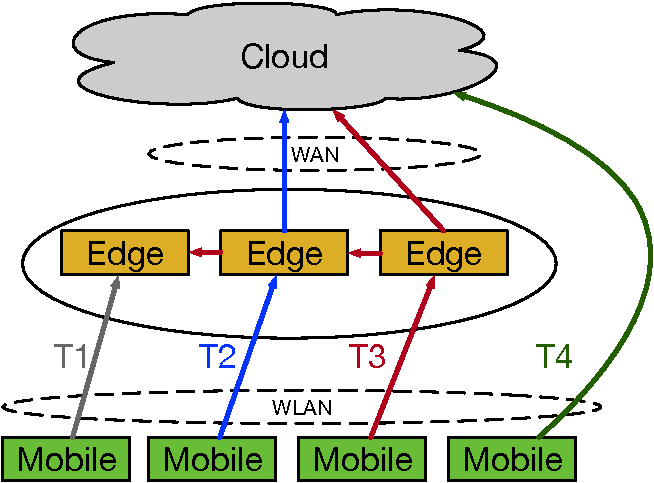
\includegraphics[width=2.5in]{Figures/computing-models.pdf}}
	\mycaption{fig-computing-models}{Computing Models}
	{
		Four different computing models under different usages of edge devices.
		Type 1 means mobile device uses one edge device only. Edge device
		can also push computation to cloud in type 2. In type 3, edge devices
		can do load-balancing. Type 4 is the original two-tier architecture,
		mobile contact with cloud only.
	}
\end{center}
\end{figure}
}

{
\begin{figure}[th]
\begin{center}
	\centerline{\includegraphics[width=2.5in]{Figures/edgecloudsim.pdf}}
	\mycaption{fig-edgecloudsim}{EdgeCloudSim Layered Architecture}
	{
		CloudSim provides the fundamental simulation support.
		Above that, EdgeCloudSim adds mobility simulation module
		and network simulation module.
	}
\end{center}
\end{figure}
}



\subsection{Computing Models}
\label{sec:computing-models}
Edge computing offers more possibilities for current mobile-cloud computing architecture.
Figure~\ref{fig-computing-models} presents four computing models. Type 4 is the original
two-tier architecture, where mobile devices communicate with cloud only. With the introduction of
edge devices, it make type 1 to type 3 possible. In type 1, mobile device contact with only one edge device.
This is benefical for mobile devices with low mobility. Compare with type 1, edge devices in type 2 can
push computation to cloud, whenever edge devices think offload can improve performance. Type 3 offers
more flexibility by load-balancing jobs among multiple edge devices.

We will evaluate type 1 to type 3 use our simulator. However, in this work we will implement our
application based on type 3 only, because we believe type 3 has better load-balaning opportunities
than others. Furthermore, type 3 is more realistic to integrate into current two-tier architecture smoothly.

\subsection{Failure Models}
\label{sec:failure-models}
While benefical from the performance aspect, edge computing also introduces more
{\em failure domains} into current computing framework. Since we are interested
in how edge devices can impact the whole performance, we will mainly focus on
the {\em additional} failure domains brought by edge computing. Namely:
\begin{enumerate}
\item Edge device crash
\item Network failure between mobile device and edge device
\item Network failure among multiple edge devices
\item Network failure between edge device and cloud
\end{enumerate}

During runtime, we assume the senders of the communication channel are able to detect failures
of receivers by software timeout. Edge devices and cloud will also use heartbeat
messages to detect liveness. Despite all these failures, the goal of resilient
edge computing is to provide high availability and reliability guarantees to
applications running on mobile devices.

\subsection{EdgeCloudSim}
Developing a set of systems softwares for edge computing is not an easy process due
to the complexity of various application requirment and different mobile devices.
Therefore it is better to have a basic understanding of what edge computing can provide
before doing real system implementation.

EdgeCloudSim~\cite{edgecloudsim} is a recent simulator designed for edge computing.
EdgeCloudSim is based on CloudSim~\cite{cloudsim}, which is a mature cloud computing simulation framework.
CloudSim is mainly designed for evaluating the performance of the data centers, thus lack the essential
properties to model edge devices and mobile devices. To be able to simulate edge computing, EdgeCloudSim
extends CloudSim by adding the following features: (i) a queueing model to represent the delay in WLAM and WAN,
(ii) a mobility model, and (iii) a new CPU utilization model for VMs~\cite{edgecloudsim}.
Figure~\ref{fig-edgecloudsim} shows its layered architecture.

EdgeCloudSim provides three different architectures: single-tier, two-tier and two-tier with load-balancing.
They map to type 1, type 2 and type 3 as illustrated in Figure~\ref{fig-computing-models} respectively.
EdgeCloudSim is also able to limit network bandwidth, simulate mobility of mobile devices.
Detailed evaluation under different settings is presented in section 3.

\section{Simulation}
\label{sec:simulation}

{
\begin{figure}[th]
\begin{center}
	\centerline{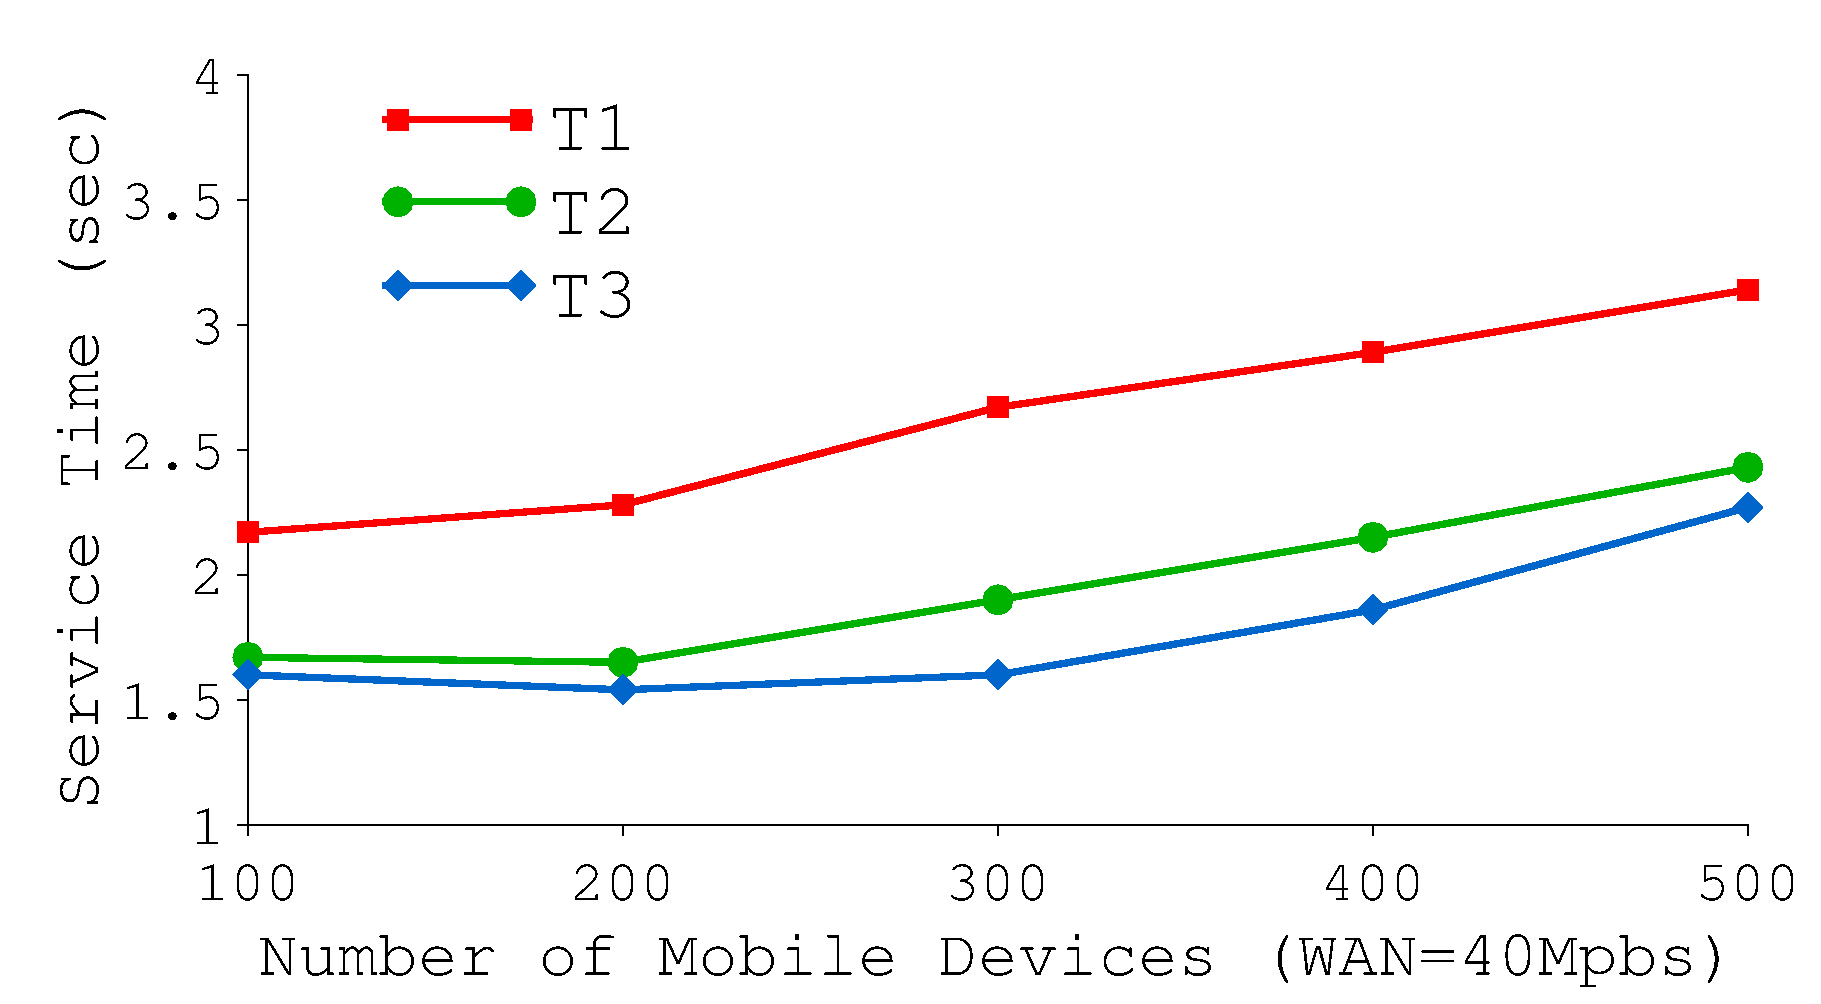
\includegraphics[width=2.5in]{Figures/g_plot_simulation-wan.pdf}}
	\mycaption{fig-simulation-wan}{Average Service Time (WAN=40Mpbs)}
	{
		T1, T2 and T3 are different computing models as described in
		Figure~\ref{fig-computing-models}. WAN bandwidth is 40Mbps,
		WLAN bandwidth is fixed 40Mbps.
	}
\end{center}
\end{figure}
}

{
\begin{figure}[th]
\begin{center}
	\centerline{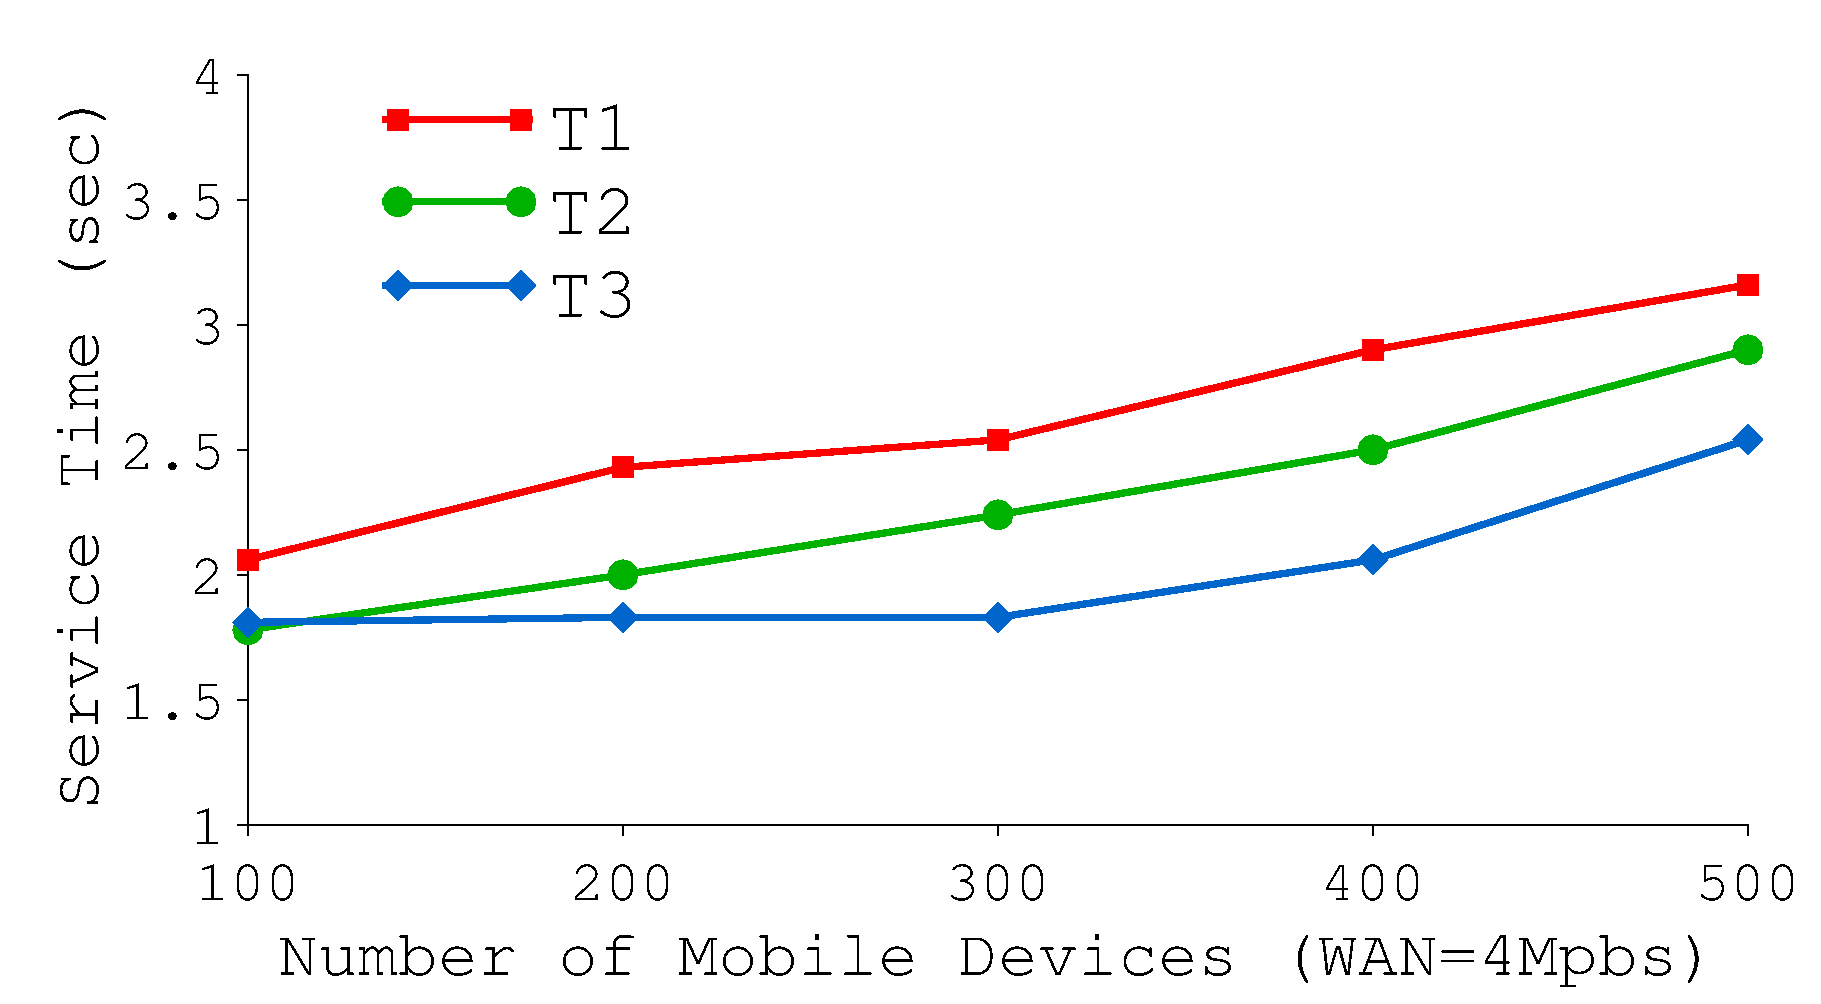
\includegraphics[width=2.5in]{Figures/g_plot_simulation-wan-4Mpbs.pdf}}
	\mycaption{fig-simulation-wan-4Mpbs}{Average Service Time (WAN=4Mpbs)}
	{
		T1, T2 and T3 are different computing models as described in
		Figure~\ref{fig-computing-models}. WAN bandwidth is 4Mbps,
		WLAN bandwidth is fixed 40Mbps.
	}
\end{center}
\end{figure}
}

The purpose of doing simulation is to have a better understanding how edge computing can
affect current mobile-cloud computing infrastructure. To put it in another way,
we ask {\em "How much better is it to offload to an edge device rather than to the cloud?"}
We focus on metrics that are important to end users, namely service time.

According to ~\cite{edgecloudsim}, the amount of time spent on WAN dominates the network delay.
Since the T1 (single-tier) model does not send tasks to the cloud, it has no WAN delay. The LAN
normally can meet user's requirment.
Figure~\ref{fig-simulation-wan} presents the average service time with 40Mpbs WAN bandwidth.
Similarly, Figure~\ref{fig-simulation-wan-4Mpbs} plots the service time while WAN only has 4Mpbs bandwidth.

It is clear that T3 has the best performance among three different computing models. Both T3 and T2 perform better
than T1 because when congestion is high, T3 and T2 can offload jobs to remote cloud. When the congestion
exceeds some threshold, T3 also has the option to offload jobs to peer edge devices.
Compare Figure~\ref{fig-simulation-wan} with Figure~\ref{fig-simulation-wan-4Mpbs}, we can find
that WAN bandwidth has little or zero effect on T1 architecture, simply because T1 does not need to offload to cloud.
With limited WAN bandwidth, both T3 and T2 has worse responsiveness. Thus it is important to maintain sufficient
bandwidth between edge devices and cloud.

\subsection{Limitation of Simulation}
Although EdgeCloudSim is able to provide average service time under different network settings and mobility settings,
the intrinsic model of using CloudSim prevents us from controlling applications in case of failures. The application
in EdgeCloudSim is described as a XML file, which lists resource (e.g., CPU, memory) requirements during runtime.
Users as us are not able to develop real applications on top of EdgeCloudSim. However, in order to achieve resilient
edge computing, we have to run mobile applications in real edge computing systems, which integrate various
fault-tolerant policies and mechanisms to provide high availability and reliability.


\section{Application}
\label{sec:application}
Real-World application, description of our android app.

\subsection{Handle Failures}
Different cases of failures, and how we handle the failure.
Testing


\section{Evaluation}
\label{sec:evaluation}

To apply the policies and mechanisms discussed in section~\ref{sec:resilient-egde},
we implemented an image-processing application on Android platform, and its edge/cloud runtime services on Linux machines.
The edge device runtime is implemented as application-specfic runtime (section~\ref{sec:policy-fault}).
Thus we have the maximum flexibity to accommodate application-specifc requirement.

\subsection{Application}
\label{sec:eval-app}

The whole system consists three parts: mobile application, edge device runtime and cloud server runtime.

\hfill\break
\noindent \textbf{Mobile Application.}
We implemented an image-processing application on Android platform. The basic functionality is to classify
whether a user-supplied image contains a hotdog or not. The core hotdog classification program is an open-source
deep learning application~\cite{url:hotdog-classification} based on TensorFlow~\cite{tensorflow-osdi}.
We can only run the hotdog classification program on Linux servers, because it is developed before the
release of TensorFlow Lite~\cite{url:tensorflow-lite}, which is TensorFlow's lightweight soluton for mobile and embedded devices.
Therefore, we will not consider running computation on the local mobile device, computation is pushed to either
edge devices or cloud servers.
In case of edge device failure, we implemented the mechanisms described in section~\ref{sec:mechanism-fault}.

\hfill\break
\noindent \textbf{Cloud Server Runtime.}
Cloud server runtime is a multithread process running on Linux servers.
It has a daemon thread keep listening for requests from either mobile or edge devices.
Besides, it also has multiple worker threads that perform image classification.
The classification is done by calling into TensorFlow runtime. Worker threads
are sleeping when no jobs are available, they will be waken up by listening thread whenever jobs arrived.
Currently, we only implement the cloud server runtime on a single machine.

\hfill\break
\noindent \textbf{Edge Device Runtime.}
Edge device runtime resembles most of logic as in cloud server runtime.
Since it is application-specific runtime, we implemented the required logic to push computation
to peer edge devices or cloud servers. We used the algorithm described in section~\ref{sec:load-balancing}
to implement load balancing. To provide high availability and reliability, we implemented the necessary
mechanisms to take over jobs that were pushed to cloud in case of WAN network failure.

\subsection{Testbed Setup}
We developed our mobile application on a Redmi 2 Pro smartphone, which has a Cortex-A53 processor, 2GB DRAM,
running with Android 4.4.4.
Our edge device is a MacBook Pro, with Intel Core i7 and 8GB DRAM. The cloud server has two Intel Xeon
E5-2620 processors, 128GB DRAM, running with CentOS 7.1 distribution and the 3.10 Linux kernel.
In our experiments, Macbook and smartphone are located at home in the same room. They connect to
the Dell server which located on Purdue campus via Xfinity network. 

\subsection{Result Analysis}
\label{sec:result-analysis}
We experiment our system with all four computing models, as described in Figure~\ref{fig-computing-models}.
For type 1 and type 2, there is only one running edge device in the system. For type 3, we deploy two
edge devices. They are running in the same Macbook, but with different ports. In type 4, mobile device
send requests to cloud server directly, no edge device is deployed. Figure~\ref{fig-app} showed the
average response time of processing a user-supplied image. The response time including both network
delay and computation time.

\hfill\break
\noindent \textbf{Base Statistics.}
In our setup, the network stays stable. The average network latency between mobile
and edge is 0.048s, mobile and server is 0.095s, edge and server is 0.07s.
The average computation time of a sinle image is 1.6s on edge, 0.48s on server.

\hfill\break
\noindent \textbf{Limitations.}
{\it a)} We upload the images from mobile device to egde device in a {\em batch fashion}, instead of
{\em streaming fashion}. Streaming uploading is more realistic in a real deployment.
The reason we choose batch fashion is due to
the huge processing gap between our smartphone, Macbook and server. If we choose to upload
images in a streaming fashion (i.e. one by one) to edge, we could only have at most
33 images on the fly based on the statistics described above. But do note that return messages
back to mobile are sent in a per-image basis.
{\it b)} The workload generated by our mobile application is not able to saturate network, our Macbook and server.
We only have one smartphone uploading images. Due to its limited processing power, it fails to create
network congestion or processing bottleneck. We even found the strong processing power imposed by our
server offsets the network gain of edge device. However, the cloud servers are normally highly utilized
in a real-world environment. The traffic created by numerous concurrent requests will saturate cloud
servers. In summary, both limitations described above are due to our simple testbed setup. If we have
more smartphones available, we believe we can have more interesting insights from experiments.

{
\begin{figure}[th]
\begin{center}
	\centerline{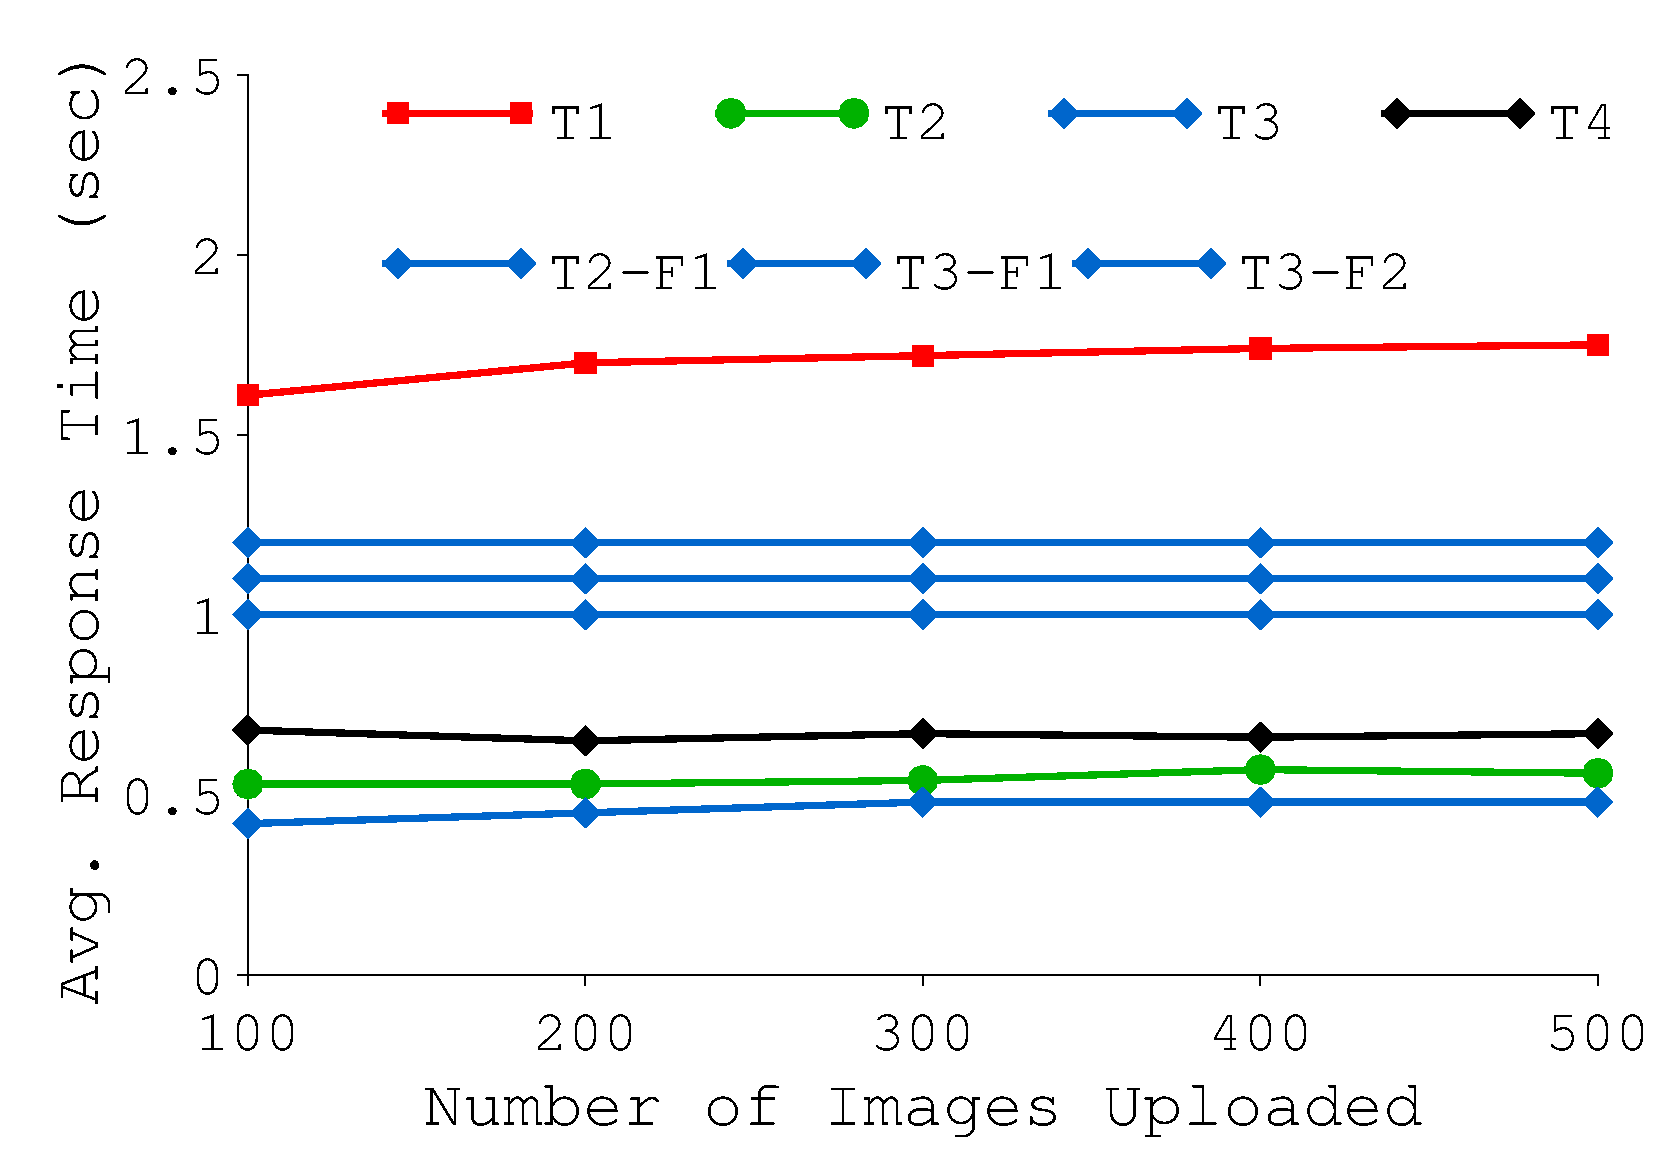
\includegraphics[width=2.5in]{Figures/g_plot_app.pdf}}
	\mycaption{fig-app}{Average Response Time Under Different Computing Models}
	{
	}
\end{center}
\end{figure}
}



\hfill\break
\noindent \textbf{Computing Models.}
Figure~\ref{fig-app} presents the average response time of a single image under different
computing models as described in section~\ref{sec:computing-models}. The average response time including: time to upload,
time for computation, possibly time for job migration, and time for return message.
Images are uploaded in a batch fashion. Computation and migration on edge device start
right after all images have been uploaded. It is clear that T3 has the best overall performance
over other computing models. This result confirms our simulation result presented in section~\ref{sec:simulation}.
T4 is better than T1 because our server has much stronger processing power than our Macbook,
which offsets the gain of edge device's fast network.
The response time of T1 and T4 stay constant even number of images increases is due to the
limitations we described above. Both T2 and T3 perform better than T4, because they have the option to
offload jobs to cloud server while having an extra parallelism on edge devices compared with T4.
In our development, T2 and T3 are using the same load-balancing algorithm described
in section~\ref{sec:load-balancing}. Due to the limitations of testbed setup, we fail to skip the
initial warmup period: migration code will calculate the best migration candidates after uploading finished,
where each edge's local copy of other \(EW\)s are all zero. Given the constant estimated run time of each job and network delay,
the percentage of jobs migrated to peer edge device or cloud stay constant too.
This explains why average response time of T2 and T3 remain constant while number of images uploaded increases.
Due to the limited time and extra engineering work needed, we are not able to present more results for after-warmup period.
We leave this for future work.

\hfill\break
\noindent \textbf{Failure Models.}
Figure~\ref{fig-app} also shows the performance comparison of T2 and T3 with failures manually injected in the middle.
The failure models follow the category of section~\ref{sec:failure-models}. T2-F1 is the case where egde device failed
during computation. T3-F1 is the case where the edge device received the uploaded images failed. T3-F2 is the case where
peer edge device failed. We emulate the edge device failure by manually killing the edge process.
Since we upload images in batch, failures must be injected after images have been uploaded while computation or migration is in progress.
Otherwise the failure of edge device will not have any effect.
Therefore, we choose to inject failure 30 seconds after images have been uploaded.
However, we don't consider cloud failure here because we envision cloud has robust failure-masking techniques.
As we described above, return messages are sent back in a per-image basis, mobile application can detect remote failures by monitoring the finished jobs.
When job failure is detected by software timeout, mobile application will resend the images again to cloud server. We choose to always resend images
back to cloud even in T3 since we did not have the mechanism to tell which edge failed.
The results in Figure~\ref{fig-app} show that even in the face of failures, T2 and T3 still have better performance than T1.
In all T2-F1, T3-F1 and T3-F2 cases, as the number of images uploaded increases,
the effect of failure increases too. This is because migration happens at the very beginning. Moreover, the time of migrating increases while number of images increases.
Thus, with a fixed failure time (i.e. 30 seconds in our testing), the number of finished jobs by the failure time descreases, which implies mobile application needs to resend more images again. This explains why the average response time increases while number of images becomes larger.

\hfill\break
\noindent \textbf{Future Work.}
Application-specifc edge device runtime requires the application developer to manage all runtime details.
Even though we have implemented the basic functionalities to achieve resilient edge computing, we still
lack several components in our system. For example, the first-run-deploy subsystem, which will help
to deploy the runtime on edge device. Also some advertising techniques for mobile devices to discover
online edge devices nearby. We are aware of the limitations in current implementation, we hope we could have
more time to extend this work.

\section{Related Work}
\label{sec:related}

\section{Conclusion}
\label{sec:conclusion}

Our study shows that edge computing..


\bibliographystyle{abbrv}
\bibliography{all-defs,all,personal,all-confs,local,paper}

\end{document}
